\chapter{Géodésiques}

Les géodésiques sont les généralisations des lignes droites de l'espace temps plat à un espace-temps courbe de métriques $g_{\mu \nu} \neq \eta_{\mu \nu}$. Elles peuvent être caractérisées de deux manières équivalentes:

\begin{theoremframe}
    \begin{defi}
    \label{def:géodésiques1}
    Les géodésiques sont
        \begin{enumerate}
            \item les courbes dont le vecteur tangent $U^\alpha = \frac{\td x^\alpha}{\td \lambda}$ est transporté parallèlement à lui-même :
            \begin{equation}
                \nabla_U U =0
            \end{equation}
            \item les courbes qui extrémisent la distance ou le temps propre entre deux points (causalement liés). 
        \end{enumerate}
    \end{defi}
\end{theoremframe}
Les géodésiques sont extrêmement importantes car elles décrivent les trajectoires de particules libres dans un espace-temps courbe c'est-à-dire en présence de gravitation\footnote{ici, "libre" signifie une particule soumis uniquement à la force gravitationnelle (et les forces d'inertie)}.

Nous considérerons en premier lieu uniquement les géodésiques temporelles, c'est-à-dire des courbes géodésiques dont le vecteur tangent est à tout point de genre temps. Nous montrerons qu'une géodésique ne peut pas changer de genre, et il suffit donc de spécifier son genre en un point. Ces courbes ont une interprétation physique immédiate via le principe d'équivalence : ce sont les trajectoires de particules libres dans une variété courbe, ou de manière équivalente, les trajectoires d'une particule dans un champ gravitationnel.

Nous généraliserons ensuite cette notion aux géodésiques nulles ($\td s^2 = 0$), et peuvent s'interpréter comme trajectoires de particules de masse nulle (p.ex. des photons). Bien que les géodésiques spatiales sont mathématiquement bien définies, ils n'apportent pas d'interprétation de trajectoires de particules physique, et ne seront donc pas abordés dans ce cours (bien qu'un développement similaire aux autres cas est possible).

\section{Géodésiques et paramétrisations}
Intéressons nous à la première définition. Soit $x^{\mu}(\lambda)$ une courbe sur une variété $(\mathcal{M}, g)$ munie de la connexion de Levi-Civita, et à vecteur tangent $U^{\mu} = \frac{dx^{\mu}}{d\tau}$. On a choisi de paramétriser la courbe par le temps propre $\tau$ qui est le temps mesuré par un·e observateur·ice "attaché·e" à la trajectoire (et donc $\td x^{i} = 0$) où pour rappel,
\begin{equation}
    \td s^2 = -\td\tau ^2 = g_{\mu \nu}\td x^{\mu}\td x^{\nu}
\end{equation}

\begin{center} 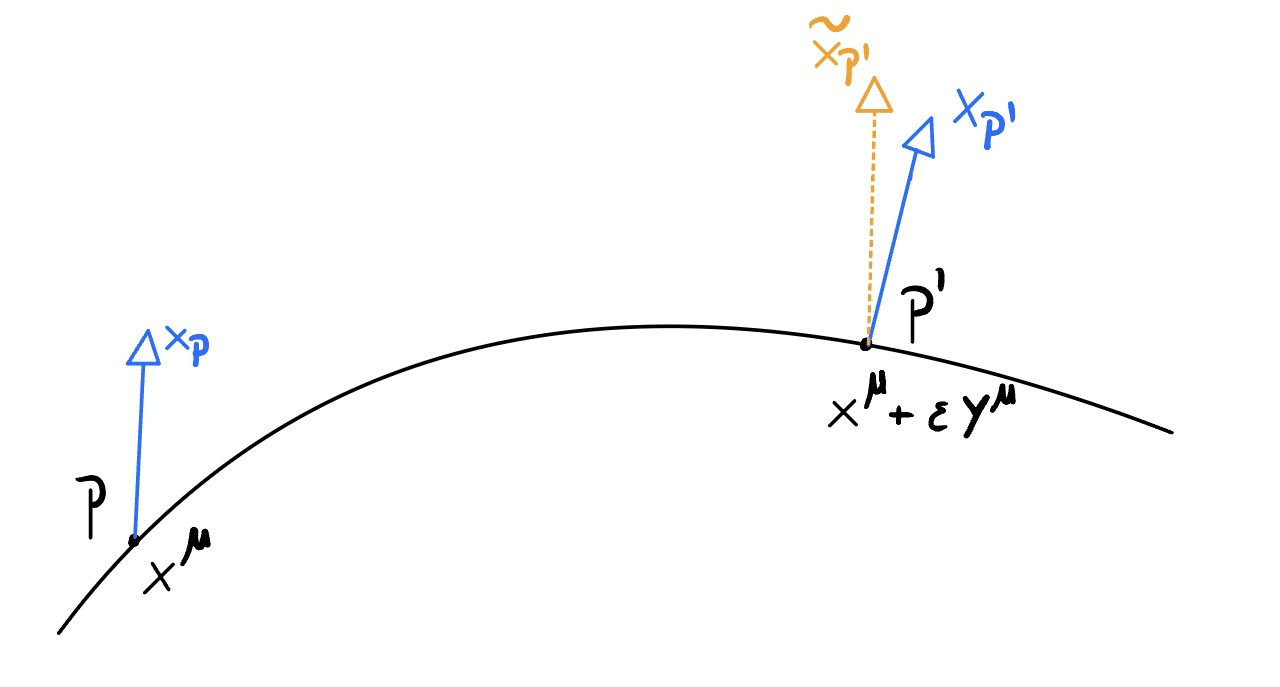
\includegraphics[scale=0.15]{Chapitres/5. Géodésiques/Images/transport parallèle.jpg} 
\end{center}

On se rappelle qu'on pouvait caractériser la connexion par le transport parallèle :
\begin{equation}
    \nabla_{Y}X = \lim_{\varepsilon \rightarrow 0}\frac{\overset{\sim}{X}(x + \varepsilon Y) - X(x+\varepsilon Y)}{\varepsilon} = 0
\end{equation}
Cette équation est nulle si et seulement si $\overset{\sim}{X}_{P'} = X_{P'}$. Le champs de vecteurs $U$ est donc bien transporté parallèlement à lui-même si et seulement si 
\begin{equation}
    \nabla_{U}U =0 
\end{equation}
Comme par la définition \ref{def:géodésiques1}. En termes de composantes,  $U = U^{\beta}\partial_{\beta}$ et donc
\begin{equation}
U^{\beta}\nabla_{\beta}U^{\alpha} = 0
\end{equation}
Autrement dit, en développant par la relation \ref{def: dérivée covariante vecteur}
\begin{align}
    &\frac{\td x^{\beta}}{\td \tau} (\partial_{\beta}U^{\alpha} + \Gamma^{\alpha}_{\beta \gamma}U^{\gamma}) = 0\\
     &\textcolor{blue}{\frac{\td x^{\beta}}{\td \tau}\frac{\partial}{\partial x^{\beta}}}\left(\frac{\td x^{\alpha}}{\td \tau}\right) + \Gamma^{\alpha}_{\beta \gamma}\frac{\td x^{\beta}}{\td \tau}\frac{\td x^{\gamma}}{\td \tau} = 0\\
     & \textcolor{blue}{\frac{\td }{\td \tau}}\frac{\td x^{\alpha}}{\td \tau} + \Gamma^{\alpha}_{\beta \gamma} \frac{\td x^{\beta}}{\td \tau}\frac{\td x^{\gamma}}{\td \tau}= 0\\
\end{align}

On obtient finalement l'\emph{équation des géodésique}s qui est aussi appelé équation des courbes \emph{auto-parallèles}:


\begin{equation}
    \boxed{\frac{\td^2x^{\alpha}}{\td\tau^2} + \Gamma^{\alpha}_{\beta \gamma}\frac{\td x^{\beta}}{\td \tau}\frac{\td x^{\gamma}}{\td \tau} = 0}
    \label{eq:géodésique} 
\end{equation}

\subsection{L'équation des géodésiques en absence de gravitation dans un référentiel inertiel}
En absence de gravitation (en relativité restreinte), $\Gamma^{\alpha}_{\mu \nu} = 0$ identiquement et donc
\begin{equation}
    \frac{\td^2x^{\alpha}}{\td\tau^2} = 0
    \label{eq:droite Minkowski}
\end{equation}
C'est l'équation d'une droite (Minkowskienne), c'est-à-dire une trajectoire du type
\begin{equation}
    x^\alpha (\tau) = v^\alpha \tau + x_0^\alpha
\end{equation}
où $v,x_0 \in \R^{3,1}$. Ce sont également les trajectoires libres usuels (en absence de gravitation et d'autres forces). En effet, l'équation \ref{eq:droite Minkowski} correspond aussi à la première loi de Newton transposée en relativité restreinte. \\
\\
Dans l'espace-temps de Minkowski, 
\begin{equation}
    \td \tau = \sqrt{\td t^2 - \td x^2 -\td y^2 - \td z^2}
\end{equation}
et donc 
\begin{equation}
    \frac{\td \tau}{\td t} = \sqrt{1- \vect{v}^2}
\end{equation}
On peut définir la quadri-vitesse selon
\begin{equation}
    u^\alpha = \frac{\td x^\alpha}{\td \tau} = \frac{\td}{\td \tau} (\td t,\td x,\td y,\td z) = \frac{1}{\sqrt{1-\vect{v}^2}} (1,\vect{v})
\end{equation}
En particulier, dans le référentiel propre de la particule, $u = (1,0,0,0)$. La quadri-accélération vaut
\begin{equation}
    a^\alpha = \frac{\td u^\alpha}{\td \tau} = \frac{\td t}{\td \tau}\frac{\td}{\td t} \lt \frac{(1,\vect{v})}{\sqrt{1-\vect{v}^2}} \rt
\end{equation}
notons $v=\lvert \vect{v} \rvert$, $\dot{v} = \frac{\td}{\td t} \lvert \vect{v} \rvert$ ainsi que $\vect{a} = \frac{\td \vect{v}}{\td t}$. On trouve alors
\begin{equation}
    a^\alpha = \lt \frac{v \dot{v}}{(1-v^2)^2}, \frac{v \dot{v}}{(1-v^2)^2} \vect{v} + \frac{1}{1-v^2} \vect{a}\rt
\end{equation}
On trouve donc que les solutions de $a^\alpha = \dfrac{\td^2 x^\alpha}{\td \tau^2} = 0$ :
\begin{equation}
    \left\{
    \begin{array}{l}
        v = 0 \quad \text{ou} \quad \dot{v} = 0  \\
        \vect{a} = 0
    \end{array}
    \right.
\end{equation}
Soit que la vitesse $\vect{v}$ de la particule est constante dans tout référentiel inertiel : la trajectoire d'une particule libre est une droite. Ceci confirme donc notre discussion ci-avant. Remarquons à présent que conformément au principe d'équivalence, \ref{eq:droite Minkowski} représente (localement) une trajectoire libre en espace-temps courbe (donc en présence de gravitation), dans un référentiel localement inertiel. \\
De la même manière, par le principê d'équivalence, \ref{eq:géodésique} représente (localement) autant la trajectoire libre dans un espace-temps courbe (donc en présence de gravitation), qu'une trajectoire libre dans un espace-temps plat, dans un référentiel non-inertiel.
\subsection{L'équation des géodésiques en absence de gravitation dans un référentiel non-inertiel}
Prenons la trajectoire d'une particule libre dans un espace-temps plat et dans un référentiel inertiel, dont l'équation du mouvement s'écrit 
\begin{equation*}
    \frac{\td^2x^{\hat{\alpha}}}{\td\tau^2} = 0
\end{equation*}
Dans un référentiel quelconque (donc non-inertiel), cette expression se transforme selon

On sait que 
\begin{align}
    \frac{\td x^{\hat{\alpha}}}{\td \tau} = \frac{\partial x^{\hat{\alpha}}}{\partial x^{\alpha}}\frac{\td x^{\alpha}}{\td\tau}
\end{align}
En différenciant une seconde fois :
\begin{align}
    0 = \frac{\td ^2x^{\hat{\alpha}}}{\td \tau^2} &= \frac{\td }{\td \tau}\left(\frac{\td x^{\alpha}}{\td \tau}\frac{\partial x^{\hat{\alpha}}}{\partial x^{\alpha}}\right)\\
    &= \frac{\td ^2x^{\alpha}}{\td \tau^2}\frac{\partial x^{\hat{\alpha}}}{\partial x^{\alpha}} + \frac{\td x^{\alpha}}{\td \tau}\frac{\td }{\td \tau}\left(\frac{\partial x^{\hat{\alpha}}}{\partial x^{\alpha}}\right)\\
    &= \frac{\td ^2x^{\alpha}}{\td \tau^2}\frac{\partial x^{\hat{\alpha}}}{\partial x^{\alpha}} + \frac{\td x^{\alpha}}{\td \tau}\frac{\td x^{\beta}}{\td \tau} \frac{\partial}{\partial x^{\beta}}\left(\frac{\partial x^{\hat{\alpha}}}{\partial x^{\alpha}}\right)\\
    &=\frac{\td ^2x^{\alpha}}{\td \tau^2}\frac{\partial x^{\hat{\alpha}}}{\partial x^{\alpha}} + \frac{\td x^{\alpha}}{\td \tau}\frac{\td x^{\beta}}{\td \tau} \frac{\partial^2 x^{\hat{\alpha}}}{\partial x^{\alpha}\partial x^{\beta}}
\end{align}
On obtient alors
\begin{align}
    0 = \frac{\partial x^{\mu}}{\partial x^{\hat{\alpha}}} \frac{\td ^2x^{\hat{\alpha}}}{\td \tau^2}&= \frac{\partial x^{\mu}}{\partial x^{\hat{\alpha}}} \left(\frac{\td ^2x^{\alpha}}{\td \tau^2}\frac{\partial x^{\hat{\alpha}}}{\partial x^{\alpha}} + \frac{\td x^{\alpha}}{\td \tau}\frac{\td x^{\beta}}{\td \tau} \frac{\partial^2 x^{\hat{\alpha}}}{\partial x^{\alpha}\partial x^{\beta}}\right)=0\\
    &=  \delta^{\mu}_{\alpha}\frac{\td ^2x^{\alpha}}{\td \tau^2} + \frac{\partial^2 x^{\hat{\alpha}}}{\partial x^{\alpha}\partial x^{\beta}}\frac{\partial x^{\mu}}{\partial x^{\hat{\alpha}}} \frac{\td x^{\alpha}}{\td \tau}\frac{\td x^{\beta}}{\td \tau}=0\\
    &= \frac{\td ^2x^{\mu}}{\td \tau^2} + \frac{\partial^2 x^{\hat{\alpha}}}{\partial x^{\alpha}\partial x^{\beta}}\frac{\partial x^{\mu}}{\partial x^{\hat{\alpha}}} \frac{\td x^{\alpha}}{\td \tau}\frac{\td x^{\beta}}{\td \tau}=0
\end{align}
En posant
\begin{equation}
    \gamma^\mu_{\alpha\beta} = \frac{\partial^2 x^{\hat{\alpha}}}{\partial x^{\alpha}\partial x^{\beta}}\frac{\partial x^{\mu}}{\partial x^{\hat{\alpha}}}
\end{equation}
On peut réécrire une équation analogue à l'équation des géodésiques pour le cas d'un espace-temps plat et dans un référentiel quelconque :
\begin{equation}
    \frac{\td ^2x^{\mu}}{\td \tau^2} + \gamma^\mu_{\alpha\beta} \frac{\td x^{\alpha}}{\td \tau}\frac{\td x^{\beta}}{\td \tau}=0
\end{equation}
Le facteur $\gamma$ joue donc le rôle des forces inertielles fictives résultantes du choix d'un référentiel non-inertiel. 
\begin{exerc}
    Montrez que dans le cas général d'un espace-temps courbe, 
    \begin{equation}
        \boxed{\Gamma^{\mu}_{\alpha \beta} = \frac{\partial^2 x^{\hat{\alpha}}}{\partial x^{\beta}\partial x^{\alpha}}\frac{\partial x^{\mu}}{\partial x^{\hat{\alpha}}} }
        \label{eq: Coefficients en dérivées}
    \end{equation}
    Ce qui confirme que les coefficients de connexion (et par extension, la métrique) capturent les forces fictives d'inertie, et par le principe d'équivalence, la gravitation.
\end{exerc}
Donnons un mode opératoire pour prouver cette égalité
\begin{enumerate}
    \item On montre que les deux objets coïncident dans un système de coordonnées particulier. 
    \item On montre que les deux côtés se transforment de la même manière sous changement général de coordonnées.
\end{enumerate}
\subsection{Paramétrisation affine}
Pour dériver l'équation des géodésiques, nous avions utilisés le temps propre comme paramétrisation de la courbe. Il s'avère que \ref{eq: Coefficients en dérivées} n'est pas invariant sous reparamétrisation de la courbe. Il est donc intéressant d'étudier une forme générale de l'équation des géodésiques où le temps propre est remplacé par un paramètre arbitraire $\lambda$. Considérons donc le changement de paramétrisation
\begin{equation*}
    x^\mu (\lambda) \to x^\mu(\tau) = x^\mu(\tau(\lambda))
\end{equation*}
Étant donné
\begin{equation}
    \frac{\td x^{\mu}}{\td \lambda} = \frac{\td \tau}{\td \lambda}\frac{\td  x^{\mu}}{\td \tau}
\end{equation}
et l'équation des géodésiques dans la paramétrisation en temps propre, on peut calculer :
\begin{align}
    \frac{\td ^2 x^{\mu}}{\td \lambda ^2} &= \frac{\td }{\td \lambda}\left(\frac{\td \tau}{\td \lambda}\frac{\td  x^{\mu}}{\td \tau}\right)\\
    & = \frac{\td ^2 \tau}{\td \lambda ^2}\frac{\td  x^{\mu}}{\td \tau} +  \frac{\td \tau}{\td \lambda} \frac{\td }{\td \lambda}\frac{\td  x^{\mu}}{\td \tau }\\
    &=\frac{\td ^2 \tau}{\td \lambda ^2}\textcolor{blue}{\frac{\td  x^{\mu}}{\td \tau}} +  \frac{\td \tau}{\td \lambda} \frac{\td \tau}{\td \lambda}\textcolor{purple}{\frac{\td ^2 x^{\mu}}{\td \tau ^2}}\\
    &= \frac{\td ^2 \tau}{\td \lambda ^2}\textcolor{blue}{\frac{\td \lambda}{\td \tau}\frac{\td  x^{\mu}}{\td \lambda}} + \left(\frac{\td \tau}{\td \lambda}\right)^2\textcolor{purple}{\lt-\Gamma^{\mu}_{\alpha \beta}\frac{\td  x^{\alpha}}{\td \tau}\frac{\td  x^{\beta}}{\td \tau} \rt}\\
    &= \frac{\td ^2 \tau}{\td \lambda ^2}\frac{\td \lambda}{\td \tau}\frac{\td  x^{\mu}}{\td \lambda} - \Gamma^{\mu}_{\alpha \beta}\frac{\td  x^{\alpha}}{\td \lambda}\frac{\td  x^{\beta}}{\td \lambda}
\end{align}
On obtient donc la généralisation suivante :
\begin{align}
     \boxed{\frac{\td ^2 x^{\mu}}{\td \lambda ^2} + \Gamma^{\mu}_{\alpha \beta}\frac{\td  x^{\alpha}}{\td \lambda}\frac{\td  x^{\beta}}{\td \lambda} = \frac{\td ^2 \tau}{\td \lambda ^2}\frac{\td \lambda}{\td \tau}\frac{\td  x^{\mu}}{\td \lambda}}
     \label{eq:pour expliquer Morera v2}
\end{align}
Une observation curieuse est que cette équation se ramène à l'équation des géodésiques précédente si et seulement si $\lambda = a \lambda + b$. Autrement dit, l'équation des géodésiques est invariante sous la reparamétrisation
\begin{equation*}
    \tau \to \lambda = a\tau+b
\end{equation*}
Un tel paramètre est appelé \emph{paramètre affine}. Notons également que seul avec un tel paramètre, les droites Minkowskiennes correspondant à des mouvements libres en relativité restreinte s'expriment sous la forme \ref{eq:droite Minkowski}.
\begin{theoremframe}
    \begin{theorem}[Théorème de je ne sais pas à quoi ça sert]
        Soit une courbe $x^\alpha (\lambda)$ à vecteur tangent $U^\alpha$ satisfaisant 
        \begin{equation}
            \nabla_U U = g(\lambda) U
        \end{equation}
        Alors il existe un changement de paramétrisation (lisse) telle que l'équation des géodésiques est satisfaite, i.e.
    \begin{equation*}
        \nabla_U U = 0
    \end{equation*}
    \end{theorem}
\end{theoremframe}
\begin{proof}
    Il suffit de considérer le raisonnement inverse qui nous a emmené à \ref{eq:pour expliquer Morera v2}. On pose alors la reparamétrisation $\lambda \to \lambda' = \lambda'(\lambda)$:
    \begin{equation}
        g(\lambda) = \frac{\td^2 \lambda'}{\td \lambda^2} \frac{\td \lambda}{\td \lambda'}
    \end{equation}
    Réécrivant les variables vers quelque chose de compréhensible, notons la nouvelle variable $q$ et l'ancienne variable $t$. On trouve alors l'EDO
    \begin{equation}
        \ddot{q}(t) g(t) = \dot{q}(t)
    \end{equation}
    Avec la fonction lisse $g$. Celle-ci admet 
\end{proof}
\section{Géodésiques et principe variationnel}
On a vu précédemment qu'on pouvait définir le genre d'une courbe (à tout point) comme le genre de son vecteur tangent en ce point. Néanmoins, dans le cas général, le genre d'une courbe peut changer en fonction du point considéré. On montre ici que ce n'est pas le cas des géodésiques
\begin{theoremframe}
    \begin{propri}
        Le genre d'une géodésique est bien défini. Autrement dit, son genre ne peut pas changer le long de la courbe. En particulier, si $\lambda$ est un paramètre affine, la norme du vecteur tangent est une constante du mouvement.
        \begin{equation}
            \frac{\td}{\td\lambda}\lVert U \rVert^2 = 0
        \end{equation}
    \end{propri}
\end{theoremframe}
Nous monterons uniquement qu'une géodésique qui est de genre temps en un point l'est à tout point. La preuve se généralise de la même manière aux autres genres.
\begin{proof}
    Soit une géodésique à coordonnées $x^{\alpha}(\lambda)$. Par le théorème ah-je-sais-à-quoi-il-sert-maintenant de la section précédente, nous pouvons sans perte de généralité considérer que celle-ci est paramétrisée par un paramètre affine à vecteur tangent  $U^{\alpha} = \frac{\td x^{\alpha}}{\td\lambda}$. Notons que le genre de la courbe à un point donné ne dépend pas du choix de paramétrisation, et il suffit donc de montrer que le genre de la géodésique est bien défini pour la paramétrisation affine. On a par définition :
    \begin{align}
        \Vert  U \Vert ^2 =& g_{\mu \nu}U^{\mu}U^{\nu}\\
        =& g_{\alpha \beta}\frac{\td x^{\alpha}}{\td \lambda}\frac{\td x^{\beta}}{\td \lambda} = g_{\alpha\beta} \dot{x}^\alpha \dot{x}^\beta
    \end{align}

    On veut montrer que 
    \begin{equation}
        \frac{\td }{\td \lambda}\left(\Vert  U \Vert ^2\right)=0
    \end{equation}
    Muni de la propriété 
    \begin{equation*}
    \frac{\td}{\td \lambda} g_{\alpha\beta} = \frac{\td x^\mu}{\td \lambda} \pd_\mu g_{\alpha\beta} = U^\mu \pd_\mu g_{\alpha\beta}
    \end{equation*}
    on calcule :
    \begin{align}
        \frac{\td }{\td \lambda}\left(\Vert  U \Vert ^2\right)
        =&\frac{\td }{\td \lambda}\left(g_{\alpha \beta}\dot{x}^{\alpha}\dot{x}^{\beta} \right)\\
        =&\left(\dot{x}^{\mu}\partial_{\mu}g_{\alpha \beta}\right)\dot{x}^{\alpha}\dot{x}^{\beta}  + 2g_{\alpha \beta}\textcolor{blue}{\ddot{x}^{\alpha}}\dot{x}^{\beta}\\
        =&\left(\dot{x}^{\mu}\partial_{\mu}g_{\alpha \beta}\right)\dot{x}^{\alpha}\dot{x}^{\beta} + 2g_{\alpha \beta}\textcolor{blue}{\left(-\Gamma^{\alpha}_{\mu \nu}\dot{x}^{\mu}\dot{x}^{\nu}\right)} \dot{x}^{\beta}\\
        =&\partial_{\mu}g_{\alpha \beta}\dot{x}^{\mu}\dot{x}^{\alpha}\dot{x}^{\beta} - 2g_{\alpha \beta}\dot{x}^{\beta}\dot{x}^{\mu}\dot{x}^{\nu}\left[\frac{1}{2}g^{\alpha \theta}\left(\partial_{\mu}g_{\theta\nu} + \partial_{\nu}g_{\mu \theta}-\partial_{\theta}g_{\mu \nu}\right)\right]
    \end{align}
    Il suffit à présent de développer le second terme 
    \begin{align}
        \frac{\td }{\td \lambda}\left(\Vert  U \Vert ^2\right)
        =&\partial_{\mu}g_{\alpha \beta}\dot{x}^{\mu}\dot{x}^{\alpha}\dot{x}^{\beta} - \dot{x}^{\theta}\dot{x}^{\mu}\dot{x}^{\nu}\left(\partial_{\mu}g_{\theta\nu} + \partial_{\nu}g_{\mu \theta}-\partial_{\theta}g_{\mu \nu}\right)\\
        =&\partial_{\mu}g_{\textcolor{blue}{\theta} \textcolor{blue}{\nu}}\dot{x}^{\mu}\dot{x}^{\textcolor{blue}{\theta}}\dot{x}^{\textcolor{blue}{\nu}} - \dot{x}^{\theta}\dot{x}^{\mu}\dot{x}^{\nu}\left(\partial_{\mu}g_{\theta\nu} + \partial_{\nu}g_{\mu \theta}-\partial_{\theta}g_{\mu \nu}\right)\\
        =&\dot{x}^{\theta}\dot{x}^{\mu}\dot{x}^{\nu}\left( \textcolor{red}{\partial_{\mu}g_{\theta\nu}} -\textcolor{red}{\partial_{\mu}g_{\theta\nu}} - \partial_{\nu}g_{\mu \theta}+\partial_{\theta}g_{\mu \nu} \right)\\
        =&\dot{x}^{\theta}\dot{x}^{\mu}\dot{x}^{\nu}\left( - \partial_{\nu}g_{\mu \theta}+\partial_{\theta}g_{\mu \nu} \right)\\
    \end{align}
    Le terme en la métrique est antisymétrique en $\nu$ et $\theta$, alors que le terme en les $\dot{x}$ en est symétrique : la contraction s'annule. 
\end{proof}
\begin{rmk}
    Le temps propre d'une courbe n'est défini que pour une courbe causale. De plus, pour les intervalles de type temps, le temps propre est identiquement nul (comme $\td s^2 = 0$) et n'est donc pas un paramètre adapté. Pour prouver le résultat ci-dessus, nous devons donc d'abord montrer que l'équation des géodésiques reste valable dans ces cas pour un paramètre affine, qui à présent sera défini comme un paramètre coupant la courbe en morceaux équidistants. La propriété principale des paramètres affines reste valable : si $\lambda$ est un paramètre affine alors $a\lambda +b$ en est un aussi.
\end{rmk}
Nous avons jusqu'ici utilisé la première version de la définition \ref{def:géodésiques1}, en définissant les géodésiques comme des \emph{courbes auto-parallèles}. Nous allons à présent nous intéresser à la deuxième formulation, en montrant qu'ils correspondent également à des \emph{courbes extrémales}. \\
\\
Nous avions vu que la longueur Minkowskienne en espace-temps plat mesurée le long de courbes causales est extrémale (maximale dans le cas présent) par la droite. Nous allons généraliser ce résultat à un espace Lorentzien quelconque $(\mathcal{M},g)$ muni de la connexion de Levi-Civita, par analogie des géodésiques comme généralisation des lignes droites.
\begin{theoremframe}
    \begin{propri}
    L'équation des géodésiques découle d'un principe variationnel : soit une courbe $x^{\mu}(\lambda)$ de genre temps. La fonctionnelle 
    \begin{equation}
        \tau[x^\mu] = \int \td\tau = \int^{\lambda_2}_{\lambda_1}\sqrt{-g_{\mu \nu}\frac{\td x^{\mu}}{\td\lambda}\frac{\td x^{\nu}}{\td\lambda}}\td\lambda
        \label{eq:principe variationnel géodésiques}
        \end{equation}
        est extrémisée par les géodésiques temporelles, c'est à dire que
        \begin{equation}
            \delta \tau = 0 \iff \frac{\td ^2 x^{\alpha}}{\td \tau^2} + \Gamma^{\alpha}_{\beta \gamma}\frac{\td x^{\beta}}{\td \tau}\frac{\td x^{\gamma}}{\td \tau} = 0
        \end{equation}
    \end{propri}
\end{theoremframe}

\begin{proof} La preuve se fait en deux étapes
    \subsubsection{Étape 1 : réécriture de la fonctionnelle}
    Posons
    \begin{equation}
        f = g_{\mu \nu}\frac{\td x^{\mu}}{\td \lambda}\frac{\td x^{\nu}}{\td \lambda}
    \end{equation}
    Alors, la fonctionnelle se réécris
    \begin{equation}
        \tau =\int^{\lambda_2}_{\lambda_1}\sqrt{-f}\td\lambda
    \end{equation}
    et sa variation s'écrit
    \begin{equation}
        \delta \tau = \int -\frac{1}{2}(-f)^{-\frac{1}{2}}\delta f \td \lambda
    \end{equation}
    Notons que l'action \ref{eq:principe variationnel géodésiques} est invariante sous reparamétrisation $\lambda \rightarrow \lambda'(\lambda)$. Choisissons donc comme paramétrisation le temps propre. On trouve alors
    \begin{equation}
        f = g_{\mu \nu}\frac{\td x^{\mu}}{\td \tau}\frac{\td x^{\nu}}{\td \tau}= \frac{\td s^2}{\td \tau ^2}= -\frac{\td \tau^2}{\td \tau ^2} = -1
    \end{equation}
    Ce qui implique que la variation du temps propre est 
    \begin{equation}
        \delta \tau = -\frac{1}{2}\int \delta f \td\tau \quad \text{donc soit} \quad \delta \tau = 0 \iff \delta f=0
    \end{equation}
    Les points stationnaires de la fonctionnelle \ref{eq:principe variationnel géodésiques} sont donc les mêmes que ceux de la fonctionnelle suivante 

    \begin{equation}
        \boxed{I[x^\mu] = \frac{1}{2}\int g_{\mu \nu} \frac{\td x^{\mu}}{\td \tau}\frac{\td x^{\nu}}{\td \tau} \td \tau \equiv \int \mathcal{L}_t \td \tau}
        \label{eq:action I}
    \end{equation}
    \subsubsection{Équations du mouvement de la nouvelle fonctionnelle}
    Sous cette forme, les équations d'Euler-Lagrange s'écrivent
    \begin{equation}
        \frac{\delta I}{\delta x^{\mu}} = 0 \iff \frac{\td }{\td \tau}\frac{\partial \mathcal{L}}{\partial \dot{x}^{\mu}} - \frac{\partial \mathcal{L}}{\partial {x}^{\mu}} = 0
    \end{equation}
Le lagrangien est
\begin{equation}
    \mathcal{L} = \frac{1}{2}g_{\alpha \beta}\dot{x}^{\alpha}\dot{x}^{\beta} 
\end{equation}
Notons que cette équation dépend bien implicitement de $x^\mu$ à travers la métrique. Calculons le termes des équations d'Euler-Lagrange :
\begin{align}
    \frac{\partial \mathcal{L}}{\partial x^{\mu}}& =\frac{1}{2}\partial_{\mu}g_{\alpha \beta}\dot{x}^{\alpha}\dot{x}^{\beta}\\
    \frac{\partial \mathcal{L}}{\partial \dot{x}^{\mu}} &= \frac{1}{2}g_{\alpha \beta}\frac{\partial \dot{x}^{\alpha}}{\partial \dot{x}^{\mu}}\dot{x}^{\beta} + \frac{1}{2}g_{\alpha \beta}\dot{x}^{\alpha}\frac{\partial \dot{x}^{\beta}}{\partial \dot{x}^{\mu}} = g_{\alpha \beta} \dot{x}^{\beta}
\end{align}
Et
\begin{align}
    \frac{\td}{\td\lambda}\frac{\partial \mathcal{L}}{\partial \dot{x}^{\mu}} &= \frac{\td}{\td\lambda}(g_{\alpha \beta}\dot{x}^{\beta})\\
    &= \dot{x}^{\gamma} \partial_{\gamma}g_{\alpha \beta}\dot{x}^{\beta} + g_{\alpha \beta}\ddot{x}^{\beta}
\end{align}
En distribuant la dérivée et en développant $\frac{\td}{\td \lambda} =\dot{x}^\mu \pd_\mu$ par la règle de la chaîne. En combinant, on trouve finalement
\begin{align}
    \partial_{\alpha}g_{\mu \nu}\dot{x}^{\alpha}\dot{x}^{\nu} + g_{\mu \nu}\ddot{x}^{\nu} - \frac{1}{2}\partial_{\mu}g_{\alpha \nu}\dot{x}^{\alpha}\dot{x}^{\nu} &= 0 \\
    \intertext{Or, comme}
    \partial_{\textcolor{purple}{\alpha}}g_{\mu \textcolor{blue}{\nu}}\dot{x}^{\textcolor{purple}{\alpha}}\dot{x}^{\textcolor{blue}{\nu}} = \frac{1}{2} \lt\partial_{\textcolor{purple}{\alpha}}g_{\mu \textcolor{blue}{\nu}} \dot{x}^{\textcolor{purple}{\alpha}}\dot{x}^{\textcolor{blue}{\nu}} + \partial_{\textcolor{purple}{\nu}}g_{\mu \textcolor{blue}{\alpha}}\dot{x}^{\textcolor{blue}{\alpha}}\dot{x}^{\textcolor{purple}{\nu}} \rt
    \intertext{On peut contracter les équations du mouvement avec $g^{\mu \beta}$}
    g^{\mu \beta} \left[\frac{1}{2}\partial_{\alpha}g_{\mu \nu} \dot{x}^{\alpha}\dot{x}^{\nu} + \frac{1}{2}\partial_{\nu}g_{\mu \alpha}\dot{x}^{\alpha}\dot{x}^{\nu} + g_{\mu \nu}\ddot{x}^{\nu} \right]  &- \frac{1}{2}\partial_{\mu}g_{\alpha \nu}\dot{x}^{\alpha}\dot{x}^{\nu} = 0\\
    \ddot{x}^{\beta} + \frac{1}{2}g^{\mu \beta} \left(\partial_{\alpha}g_{\mu \nu} + \partial_{\nu}g_{\mu \alpha} - \partial_{\mu}g_{\alpha \beta}\right) \dot{x}^{\alpha}\dot{x}^{\nu} &= 0
\end{align}
On peut directement définir les coefficients de connexion via l'expression \ref{Connexion de Levi-Civita}.
\begin{equation}
    \frac{d^2x^{\alpha}}{d\lambda^2 } + \Gamma^{\mu}_{\alpha \beta} \frac{dx^{\alpha}}{d\lambda} \frac{dx^{\beta}}{d\lambda} = 0
\end{equation}
Les courbes auto-parallèles et les courbes qui extrémisent le temps propre sont les mêmes et sont valables pour tout $\Gamma$.
\end{proof}
Formulons une série de commentaires sur cette propriété :
\begin{enumerate}

    \item La fonctionelle $\tau[x^\mu]$ est invariante sous reparamétrisation alors que $I[x^\mu]$ ne l'est pas. Ce n'est que lorsque les courbes sont paramétrés par un paramètre affine que les points stationnaires des actions [\ref{eq:temps propre}] et [\ref{eq:action I}] coïncident. En effet, si les courbes sont paramétrés par $\lambda = a\tau + b$  on obtient que  $\td\tau = a \td\lambda$ et 
    \begin{equation}
    \frac{\td}{\td\tau} = \frac{\td\lambda}{\td\tau}\frac{\td}{\td\lambda} = \frac{1}{a}\frac{\td}{\td\lambda}
    \end{equation}
    La fonctionelle $I$ se transforme donc sous un paramètre affine selon
    \begin{equation}
        I \to \frac{1}{2}\int g_{\mu \nu}\frac{1}{a^2}\frac{\td x^{\mu}}{\td\lambda}\frac{\td x^{\nu}}{\td\lambda} a \,\td\lambda = \frac{1}{a}I
    \end{equation}
    On voit que manifestement, $I$ n'est pas invariant sous changement de paramétrisation, et n'aura en général plus les mêmes points stationnaires.
    \item Pour une conexion de Levi-Civita, les courbes auto-parallèles coïncident avec les courbes extrémales (maximales) du temps propre. Ceci est important pour que le principe d'équivalence soit vrai.
    \item L'équation des géodésiques sont des équations du second ordre. Une géodésique est donc caractérisé par deux données initiales comme par exemple :
    \begin{equation}
        x^\mu(P) \quad \text{et} \quad \frac{\td x^\mu}{\td \lambda} (P)
    \end{equation}
    ou encore
    \begin{equation}
        x^\mu(P) \quad \text{et} \quad x^\mu(Q)
    \end{equation}
    En particulier, s'il existe un point $P$ tel que deux géodésiques possèdent le même vecteur tangent en ce point, alors elles sont identiques (unicité de la solution au problème de Cauchy). 
    \item En un point, il peut y avoir trois types différents de géodésique.
\end{enumerate}
En conclusion à cette partie, les observateurs en chute libre (observateurs localement inertiels) suivent une géodésique. Leur quadri-accélération est nulle. En effet, ceux-ci sont supposés uniquement soumis à la gravitation, et se meuvent donc en chute libre dans un espace-temps courbe selon le principe d'équivalence.

\section{Géodésiques nulles*}
\section{Observateurs localement inertiels revisités}
Nous allons retravailler la formulation du principe d'équivalence dans le cadre des géodésiques (qui sont les RLI prédits par celui-ci).
\begin{theoremframe}
    \begin{theorem}
        Soit une géodésique de genre temps. Il existe au moins un système de coordonnée $\{x^{\mu}\} = \{x^0 , x^k\}$ tel que le long de la géodésique :
        \begin{enumerate}
            \item $x^k = 0$
            \item $\tau = x^0$ 
            \item $g_{\alpha \beta}(x^0, 0) = \eta_{\alpha \beta}$
            \item $\Gamma^{\alpha}_{\beta \gamma}(x^0, 0) = 0$
        \end{enumerate}
    \end{theorem}
\end{theoremframe}
\begin{proof}
    Une partie de la preuve sera abordée en séance d'exercices.
    \subsubsection{Preuve de la propriété 1.}
    Soit $y^{\mu}(\tau)$ une géodésique. Son équation est donné par 
    \begin{equation}
        \left\{
        \begin{array}{l}
            y^0 = y^0(\tau)\\
            y^{i} = y^{i}(\tau)
        \end{array}
        \right.
    \end{equation}
    Comme le vecteur tangent de la géodésique ne s'annule jamais (comme c'est une géodésique temporelle), nous pouvons appliquer le \emph{théorème de la fonction implicite}. Celui-ci assure qu'on peut inverser localement l'équation $y^0 = y^0(\tau)$ en tout point tel que $\tau = \tau(y^0)$ (ainsi, on peut l'inverser globalement). En injectant cette relation dans la partie spatiale : 
    \begin{equation}
        y^{i} = y^{i}(\tau(y^0)) = y^{i}(y^0)
    \end{equation}
    On peut introduire un nouveau système de coordonnée tel que
    \begin{equation}
        \left\{
        \begin{array}{l}
            \Bar{x}^k = y^k - y^k(y^0)=0\\
            \Bar{x}^0 = y^0
        \end{array}
        \right.
    \end{equation}
    Ceci est valable pour tout observateur.

    \subsubsection{Preuve de la propriété 2.}
    Le temps propre est défini par $\td \tau ^2 = -\td s^2 = -g_{\mu \nu}\td x^{\mu} \td x^{\nu}$. Le long d'une géodésique, dans les coordonnées $\Bar{x}^k$ de la preuve précédente, on trouve
    \begin{equation}
        \td \tau ^2 = -g_{0 0}(\Bar{x}^0, 0)\td \Bar{x}^{0} \td \Bar{x}^{0}
    \end{equation}
    Donc $\tau = \tau(\Bar{x}^0)$. On cherche un nouveau système de coordonnées $x'^k$ tel que la propriété 1. reste satisfaite et l'équation $\td \tau^2 = - g_{00}(\Bar{x}^0)(\td \Bar{x}^0)^2$ devient $(\td x'^0)^2$. Comme la métrique dépend uniquement de $\Bar{x}^0$, il suffit d'effectuer la transformation
    \begin{equation}
        \left\{
        \begin{array}{l}
            x'^0 = \tau(\Bar{x}^0)\\
            x'^k = \Bar{x}^k
        \end{array}
        \right.
    \end{equation}
    Alors le temps propre le long de la géodésique $x'^{\mu} = x'^{\mu}(\tau)$ est $\tau = x'^{0}$.

    \subsubsection{Preuve de la propriété 3.}
    Le système de coordonnées précédent implique directement que la composante temporelle de la métrique $g_{00}$ se ramène à $-1$ dans le système de coordonnées $x'^\mu$. Nous cherchons donc un nouveau système de coordonnées $\Tilde{x}^\mu$ dans lequel les conditions \emph{(i)}, \emph{(ii)} et \emph{(iii)} sont satisfaites : 
    \begin{equation}
        \left\{
        \begin{array}{l}
            x'^0 = \Tilde{x}^0 + L\indices{^0_k}(\Tilde{x}^0) \Tilde{x}^k\\
            x'^k = \tilde{x}^k
        \end{array}
        \right.
    \end{equation}
    La condition \emph{(i)} reste manifestement vérifiée. La condition \emph{(ii)} impose 
    \begin{equation}
        \td \tau^2 = - g_{\tilde{0} \tilde{0}} (\td \tilde{x}^0)^2
    \end{equation}
    Par la loi de transformation de la métrique :
    \begin{align}
        \tilde{g}_{0 0} = \frac{\pd x^{\mu'}}{\pd \tilde{x}^0} \frac{\pd x^{\nu'}}{\pd \tilde{x}^0} g_{\mu'\nu'} = \dots =  g_{0'0'}
    \end{align}
    D'après un petit calcul que vous pouvez vérifier vous-même (similaire à la procédure ci-dessous). Imposons donc que la condition \emph{(iii)} soit également respectée
    \begin{align}
        \tilde{g}_{0i} &= \left. \frac{\pd x^{\mu'}}{\pd \tilde{x}^0} \frac{\pd x^{\nu'}}{\pd \tilde{x}^i}g_{\mu'\nu'} \right|_{\tilde{x}^k =0}\\
        & = \blue{\frac{\pd x^{0'}}{\pd \tilde{x}^0}} \frac{\pd x^{0'}}{\pd \tilde{x}^i}g_{0'0'} + \blue{\frac{\pd x^{0'}}{\pd \tilde{x}^0} }\gray{\frac{\pd x^{j'}}{\pd \tilde{x}^i}}g_{0'j'} +\purple{\frac{\pd x^{j'}}{\pd \tilde{x}^0}} \frac{\pd x^{0'}}{\pd \tilde{x}^i}g_{j'0'} + \purple{\frac{\pd x^{j'}}{\pd \tilde{x}^0}} \frac{\pd x^{k'}}{\pd \tilde{x}^i}g_{j'k'}
        \intertext{Où les termes en rouge s'annulent en considérant la transformation choisie. Les termes en bleu donnent 1 et le terme en gris donne $\delta^{j'}_i$.}
        &= \frac{\pd x'^{0}}{\pd \tilde{x}^i}g'_{00} +  g'_{0i} = -L\indices{^{0}_i} +  g'_{0i}
    \end{align}
    Nous pouvons ainsi imposer la condition :
    \begin{equation}
        L\indices{^0_i}(\tilde{x}^0) = \left. g'_{0i} \right|_{x'^k = 0}
    \end{equation}
    Pour que la métrique se simplifie selon $\left. \tilde{g}_{0i} \right|_{\tilde{x}^k = 0} = 0$. Il reste donc à diagonaliser $\tilde{g}_{ij}$. Considérons donc une nouvelle base de coordonnées\footnote{J'ai malheureusement épuisé mon arsenal de symboles sympas : good luck with this shit} $\{\mathfrak{z}^\mu \}$ tel que
    \begin{equation}
        \left\{
        \begin{array}{l}
            \tilde{x}^0 = \mathfrak{z}^0\\
            \tilde{x}^k = L\indices{^k_m}(\mathfrak{z}^0) \cdot \mathfrak{z}^m
        \end{array}
        \right.
    \end{equation}
    On peut toujours diagonaliser la matrice symétrique $\tilde{g} \to \mathfrak{g}$ par une matrice orthogonale $L$. Ensuite, nous pouvons normaliser séparément les $\mathfrak{z}^i \to \lambda^{(i)} \mathfrak{z}^i $ pour que ces coefficients soient égaux à 1\footnote{Notons que ceci ne modifiera pas les propriétés \emph{(i)} et \emph{(ii)}.}. Ceci conclut la preuve de la propriété \emph{(iii)}. 
\subsubsection{Preuve de la propriété 4.}
La preuve sera effectué en TP. Notons néanmoins que la preuve nécessitera le fait que la courbe $\mathfrak{z}^\mu(\mathfrak{z}^0)$ satisfait à l'équation des géodésiques.
\end{proof}
Notons que les propriétés \emph{(i)}-\emph{(iii)} n'ont pas nécessité l'hypothèse que la courbe est une géodésique. Elles restent donc vrai pour un observateur acceléré. N
\section{La limite Newtonienne}
Dans la limite Newtonienne (où $v \ll c$), nous aimerions imposer que l'équation des géodésiques se ramène à la loi de gravitation Newtonienne. Soit donc l'équation des géodésiques dans une métrique Lorentzienne arbitraire (courbe)
\begin{equation}
    \frac{d^2x^{\mu}}{d\tau^2} + \Gamma^{\mu}_{\alpha \beta}\frac{dx^{\alpha}}{d\tau}\frac{dx^{\beta}}{d\tau} = 0
\end{equation}
Dans cette limite, nous souhaitons retrouver 
\begin{equation}
    \sum \vect{F} = m\vect{a} = m\vect{g} = -m\vect{\nabla}\Phi
\end{equation}
où $\Phi$ est le potentiel gravitationnel :
\begin{equation}
\left\{
\begin{array}{l}
\Vec{g} = -\frac{GM}{r^2}.\Vec{1_{r}}\\
\Phi = \frac{GM}{r}
\end{array}
\right.
\end{equation}
En composantes, nous pouvons réécrire ceci comme
\begin{equation}
    \frac{d^2x^{i}}{dt^2} = -\partial^{i}\Phi
\end{equation}

\subsection{Gravitation linéarisée et limite newtonienne}
La limite Newtonienne, également appelée la gravitation linéarisée se définit comme suit :
\begin{theoremframe}
    \begin{defi} 
    La limite Newtonienne est
    \begin{enumerate}
        \item $\dfrac{\td x^{i}}{\td t} \ll c = 1$
        \item $g_{\mu \nu} = \eta_{\mu \nu} + h_{\mu \nu} + O(h^2)$ où $h$ représente une petite correction à la métrique plate. 
        \item $\partial_0 g_{\mu \nu} = 0$ i.e. le champ gravitationnel est statique (ne change pas dans le temps). Cela signifie aussi qu'aucune coordonnée ne dépend du temps. 
    \end{enumerate}
    \end{defi}
\end{theoremframe}
On va implémenter ces 3 conditions dans l'équation des géodésiques. Considérons $x^0 = ct$. Par \textit{(1)}, on a que 
\begin{align}
    \frac{dx^{i}}{dt} = \frac{dx^{i}}{dx^0} \ll 1 \implies \frac{dx^{i}}{d\tau} \ll \frac{dx^{0}}{d\tau}
\end{align}
Les termes en $\dfrac{dx^{i}}{d\tau}$ sont donc d'ordre supérieur et seront négligés dans la suite.
\begin{equation}
     \frac{\td ^2x^{\mu}}{\td \tau^2} + \Gamma^{\mu}_{0 0}\left(\frac{\td x^{0}}{\td \tau}\right)^2 +\dots = 0
\end{equation}
Que vaut $\Gamma^{\mu}_{0 0}$?
\begin{align}
    \Gamma^{\mu}_{0 0} &= \frac{1}{2}g^{\alpha \mu}(\partial_0 g_{\alpha 0} + \partial_{0}g_{0\alpha} - \partial_{\alpha}g_{00})\\
    &= -\frac{1}{2}g^{\alpha \mu}\partial_{\alpha}g_{00}
\end{align}
Où les deux premiers termes s'annulent par \textit{(3)}. 
De plus, par \textit{(2)}, $g_{\mu \nu} = \eta_{\mu \nu} + h_{\mu \nu} + O(h^2)$.
\begin{equation}
    \Gamma^{\mu}_{0 0} =-\frac{1}{2}g^{\alpha \mu}\partial_{\alpha}h_{00}
\end{equation}
Si $g_{\mu \nu} = \eta_{\mu \nu} + h_{\mu \nu} +O(h^2)$, alors $g^{\mu \nu} = \eta^{\mu \nu} - h^{\mu \nu } +O(h^2)$ (via la relation $g^{-1} g = \mathrm{Id}$). On trouve alors
\begin{align}
    \Gamma^{\mu}_{0 0} &=-\frac{1}{2}(\eta^{\mu \alpha} - h^{\mu \alpha })\partial_{\alpha}h_{00}\\
    &= -\frac{1}{2}\eta^{\mu \alpha}\partial_{\alpha}h_{00}\\
\end{align}
car on néglige les termes en $h^2$. L'équation des géodésique à la limite newtonienne s'écrit donc
\begin{equation}
     \frac{\td ^2x^{\mu}}{\td \tau^2} -\frac{1}{2}\eta^{\mu \alpha}\partial_{\alpha}h_{00}\left(\frac{\td x^{0}}{\td \tau}\right)^2 = 0
\end{equation}
Pour $\mu = 0$ :
\begin{align}
     &\frac{\td ^2x^{0}}{\td \tau^2} -\frac{1}{2}\eta^{00}\partial_{0}h_{00}\left(\frac{\td x^{0}}{\td \tau}\right)^2 = 0\\
\end{align}
Par \textit{(3)}, on a que $\partial_{0}h_{00} =0$.
\begin{equation}
    \frac{\td ^2x^{0}}{\td \tau^2} = 0 \implies \frac{\td x^{0}}{\td \tau} = \text{cste}
\end{equation}
i.e. on retrouve que $t$ est un paramètre affine, et on impose $ct = \tau$.
Pour $\mu = i$ :
\begin{align}
     &\frac{\td ^2x^{i}}{\td \tau^2} -\frac{1}{2}\partial^{i}h_{00}\left(\frac{\td x^{0}}{\td \tau}\right)^2 = 0\\
\end{align}
Or, par la chaîne :
\begin{align}
    \frac{\td }{\td \tau} = \frac{\td x^{\mu}}{\td \tau} \partial_{\mu}& = \frac{\td x^{0}}{\td \tau} \partial_{0} + \frac{\td x^{k}}{\td \tau} \partial_{k}\\
    & \simeq \frac{\td x^{0}}{\td \tau} \partial_{0}
\end{align}
Par \textit{(1)}. On reparamétrise la courbe avec $x^0(\tau)$ :
\begin{align}
     \frac{\td^2 x^{i}}{\td \tau^2} &= \frac{\td \textcolor{purple}{x^{0}}}{\td \tau} \partial_{\textcolor{purple}{0}}\left( \frac{\td \textcolor{blue}{x^{0}}}{\td \tau} \frac{\td x^{i}}{\td \textcolor{blue}{x^0}}\right)\\
     &=\frac{\td x^{0}}{\td \tau} \frac{\td x^{0}}{\td \tau}\partial_{0}\left(\frac{\td x^{i}}{\td x^0}\right) \\
     &=\left(\frac{\td x^{0}}{\td \tau}\right)^2 \frac{\td }{\td x^0}\left(\frac{\td x^{i}}{\td x^0}\right)\\
     &=\left(\frac{\td x^{0}}{\td \tau}\right)^2 \frac{\td ^2 x^{i}}{\td (x^0)^2}
\end{align}
La composant $\mu = i$ s'écrit donc
 \begin{align}
     \left(\frac{\td x^{0}}{\td \tau}\right)^2 \frac{\td ^2 x^{i}}{\td (x^0)^2} -\frac{1}{2}\partial^{i}h_{00}\left(\frac{\td x^{0}}{\td \tau}\right)^2 = 0\implies \frac{\td ^2 x^{i}}{\td (x^0)^2} -\frac{1}{2}\partial^{i}h_{00}=0
\end{align}
On réstore $c$ à travers $x^0 = ct$ :

\begin{align}
   \frac{1}{c^2} \frac{\td ^2 x^{i}}{\td t^2} -\frac{1}{2}\partial^{i}h_{00}=0\implies \frac{\td ^2 x^{i}}{\td t^2} = \frac{c^2}{2}\partial^{i}h_{00}
\end{align}

Comme $\frac{\td ^2 x^{i}}{\td t^2} = -\partial^{i}\Phi$ par Newton, on impose
\begin{align}
    &h_{00} = -\frac{2}{c^2}\Phi\\
    &\boxed{g_{00} = -\left(1 + \frac{2\Phi}{c^2}\right)}
\end{align}
Par conséquent, la courbure de l'espace-temps (manifestée à travers une métrique non-triviale) permet de décrire la gravité dans la limite newtonienne pour autant que la métrique soit de la forme $g_{00} = -\left(1 + \frac{2\Phi}{c^2}\right)$.

\subsection{Redshift gravitationnel}

On avait vu précédemment qu'une des conséquence du principe d'équivalence est que la fréquence et le temps propre varie en fonction de la hauteur dans lequel on se trouve dans le champ de gravitation. Donc un photon qui se propagent dans un champ de gravitation était décalé vers le rouge lorsqu'il s’élève dans celui-ci. 

\begin{center} 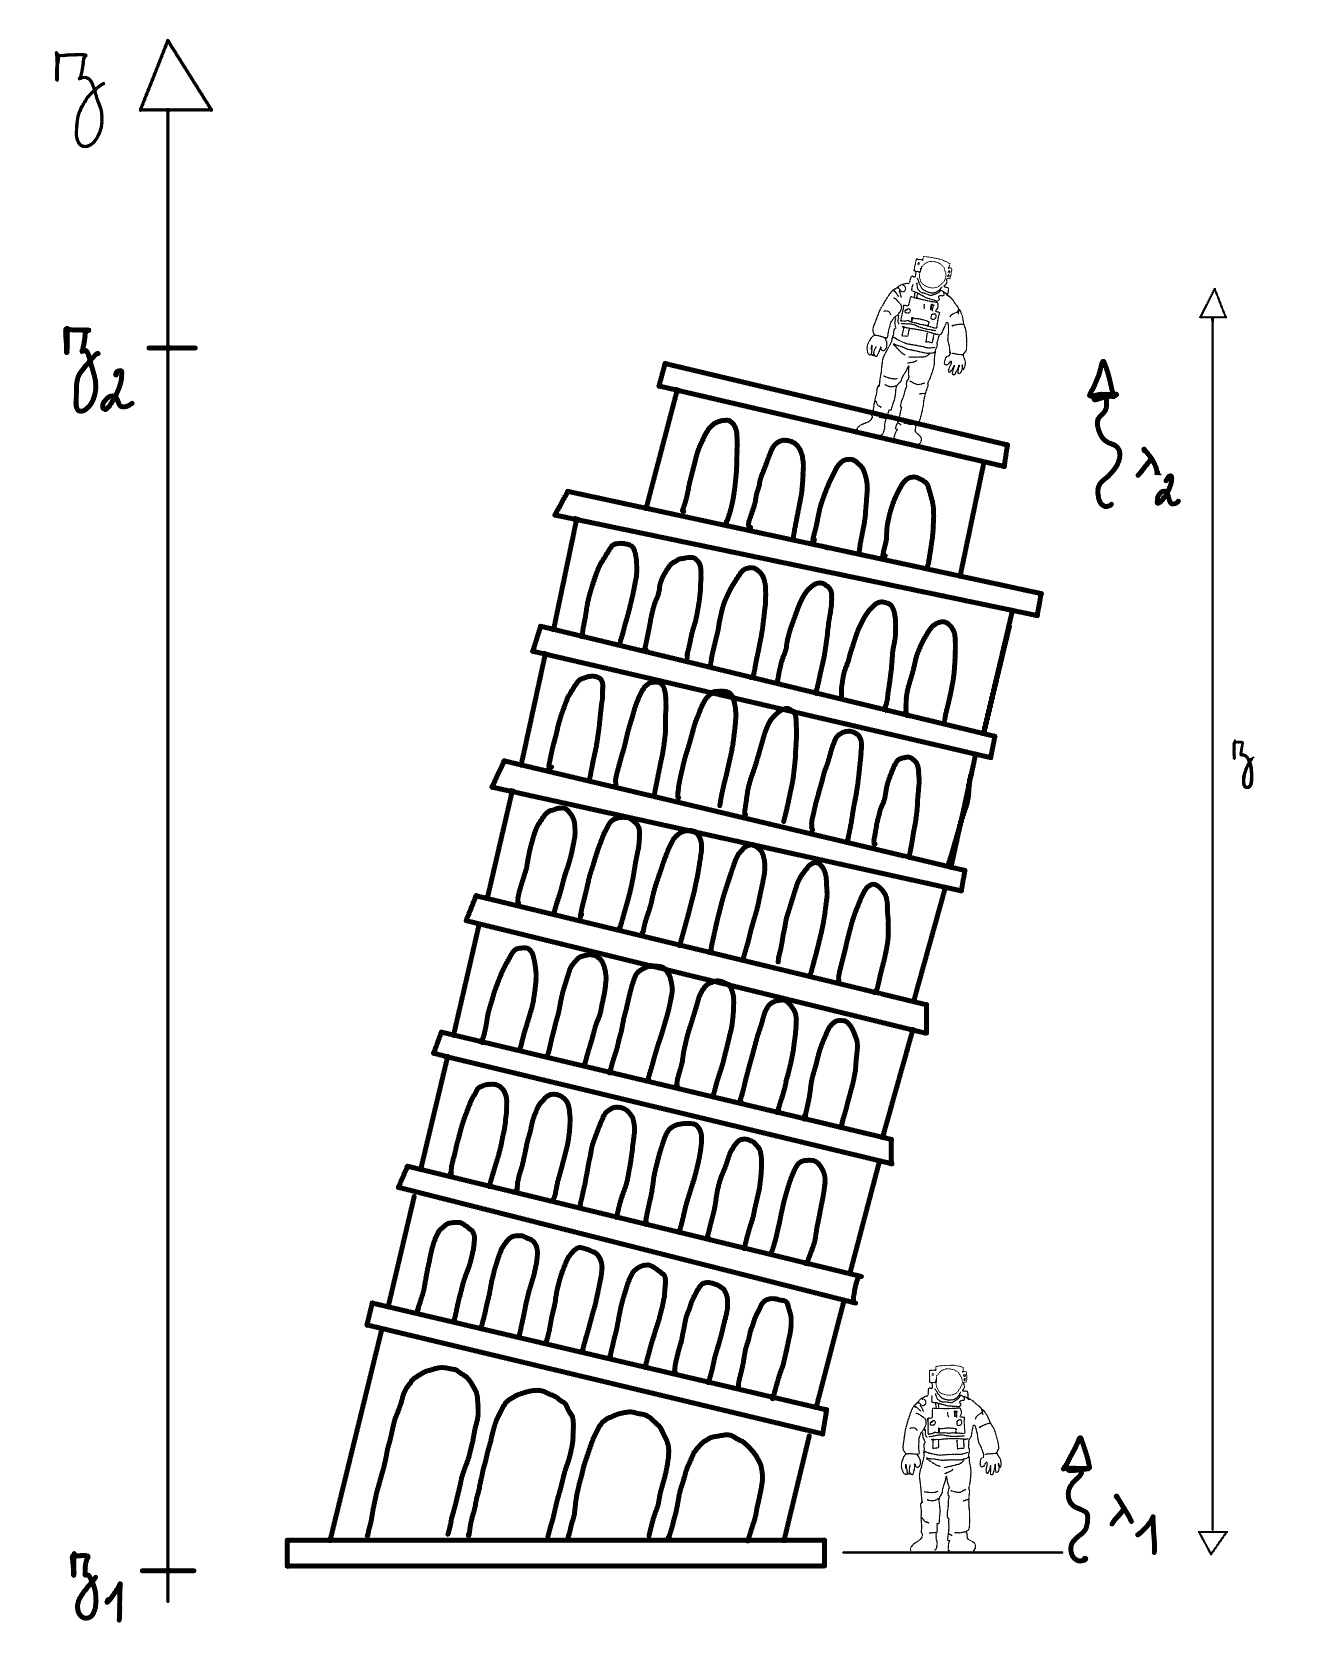
\includegraphics[scale=0.15]{Chapitres/5. Géodésiques/Images/tour de pise.jpg} 
\end{center}

On considère que le champ gravitationnel est statique (indépendant du temps). Les trajectoires $AB$ et $CD$ sont parallèles (cf. ci-dessous). Donc $\td t_{E} = \td t_{R}$. Ceci nous avait troublé parce qu'en espace temps plat, $\td t_{E} = \td t_{R}$ implique que $T_E = T_R \Leftrightarrow \lambda_E \Leftrightarrow \lambda_R$. Or le principe d'équivalence prédit un redshift, qui de plus a été mesuré. Nous allons voir pourquoi il n'y a pas de contradiction. La résolution se trouve dans le fait qu'en présence de gravitation (faible), la métrique n'est plus plate mais décrite par $g_{00} = -\left(1 + \frac{2\Phi}{c^2}\right)$.

\begin{center} 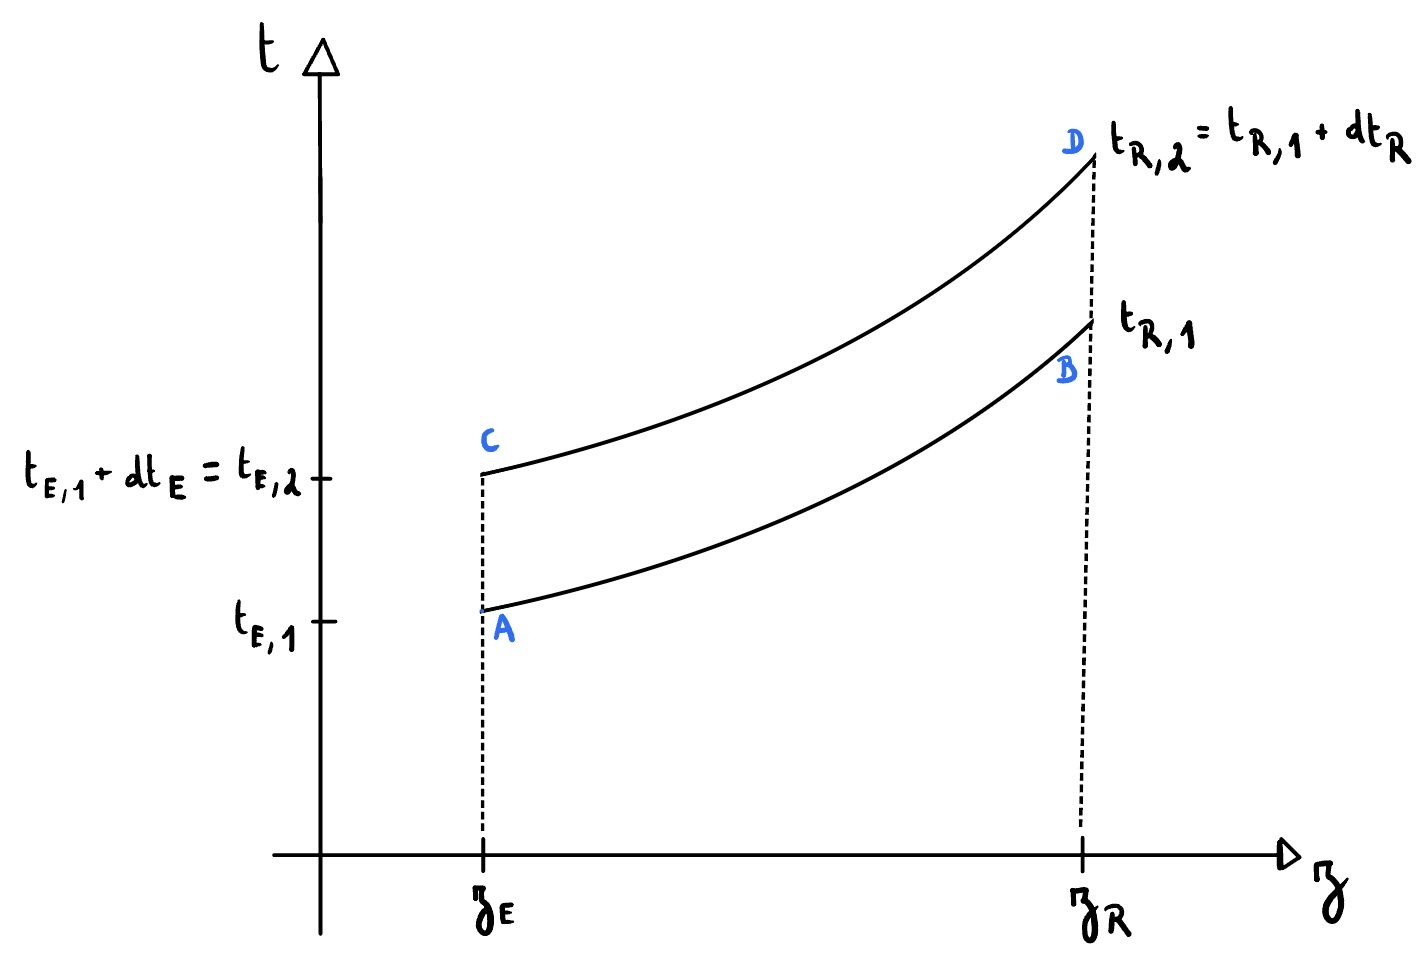
\includegraphics[scale=0.15]{Chapitres/5. Géodésiques/Images/redshift.jpg}  
\end{center}

Le rapport des longueurs d'ondes est donné par 

\begin{equation}
    \frac{\Delta \lambda}{\lambda} = \frac{\lambda -\lambda_0}{\lambda} = \frac{gz}{c^2}=\frac{\Delta \Phi}{c^2}
\end{equation}
où $\vect{g} = -\frac{GM}{r^2}.\vect{1_{r}}$, $\Phi = \frac{GM}{r}$, $\lambda > \lambda_0$, $t_{E, 1}$ est le temps d'émission de la première onde et $t_{E, 2}$ est le temps d'émission de la deuxième onde. 

Le temps propre à l'endroit de l'émission est 
\begin{align}
    \td \tau_E^2 &= -g_{\mu \nu}|_{z_E}\td x^{\mu}\td x^{\nu}\\
    &= - g_{0 0}(z_E)\td t^2_E
\end{align}
Et le temps propre à l'endroit de la réception est 
\begin{align}
    \td \tau_E^2 = - g_{0 0}(z_R)\td t^2_R
\end{align}
Donc même si les intervalles $\td t_E$, $\td t_R$ sont les mêmes (champ statique), les temps propres ne sont pas les mêmes. C'est ces temps propres que les observateurs ont mesuré. 

\begin{equation}
    \frac{\td \tau_E}{\td \tau_R} = \sqrt{\frac{g_{00}(z_E)}{g_{00}(z_R)}}
\end{equation}
car $\td t^2_E = \td t^2_R$. En remplaçant par l'expression de la métrique :


\begin{equation}
     \frac{\td \tau_E}{\td \tau_R} = \sqrt{\frac{1+\frac{2\Phi(z_E)}{c^2}}{1+\frac{2\Phi(z_R)}{c^2}}}
\end{equation}
Comme on suppose que le champ gravitationnel est faible, $\frac{2\Phi(z_E)}{c^2} << 1$, qu'on peut donc développer au premier ordre 

\begin{align}
     \frac{\td \tau_E}{\td \tau_R} = \frac{T_E}{T_R} = \frac{\lambda_E}{\lambda_R} &\simeq \lt 1 +\frac{\Phi(z_E)}{c^2}\rt \lt 1-\frac{\Phi(z_R)}{c^2} \rt\\
     & \simeq 1 - \frac{\Delta \Phi}{c^2}
\end{align}

où $\Delta\Phi = \Phi(z_R) - \Phi(z_E)$. On obtient donc un redshift

\begin{align}
    \frac{\Delta \lambda}{\lambda_R} = 1 - \frac{\lambda_E}{\lambda_R} &= \frac{\Delta\Phi}{c^2}  \\
    &= \frac{GM}{c^2}\lt\frac{1}{R} -\frac{1}{R+z}\rt\\
    &= \frac{GM}{c^2}\lt \frac{R + z - R}{R(R+z)}\rt\\
    & \Delta \frac{GM}{c^2 R^2}z\\
    &=\frac{gz}{c^2}
\end{align}
Donc on trouve que 
\begin{equation}
    \frac{\nabla \lambda}{\lambda} = \frac{gz}{c^2}
\end{equation}
Qui est exactement ce qu'on avait précédemment. Donc la métrique courbe peut expliquer les effets non triviaux dans un champ de gravitation. La métrique courbe explique donc le redshift gravitationnel. 

\section{Déviation des géodésiques et tenseur de Riemann}

Le principe d'équivalence nous a appris que localement les effets d'un champ de gravitation peuvent être annulés en se plaçant dans des coordonnées localement inertielles, qui correspond au référentiel d'un observateur en \emph{chute libre}. Ceci s'était traduit mathématiquement par le fait d'avoir non-seulement $g_{\mu \nu} = \eta_{\mu \nu}$ et $\partial_{\alpha}g_{\mu \nu} = 0 = \Gamma^{\alpha}_{\beta \gamma}$ en un point, mais aussi le long de toute géodésique de genre temps pour des coordonnées bien choisies. Par conséquent, pour détecter la présence d'un champ de gravitation, une seule géodésique (un seul observateur) ne suffit pas. Il faut étudier comment les géodésiques voisines se comportent les unes par rapport aux autres. 

Un postulat fondamental de la géométrie euclidienne, c'est-à-dire de l'espace-temps plat, est que les droites (c'est-à-dire des géodésiques de cet espace) initialement parallèles le restent. En espace-temps courbe c'est-à-dire en présence de gravitation, deux droites peuvent s'intercepter. Cet effet est facilement illustré sur la sphère. Des géodésiques initialement parallèle sur une sphère vont finir par s'intercepter. 

\begin{center} 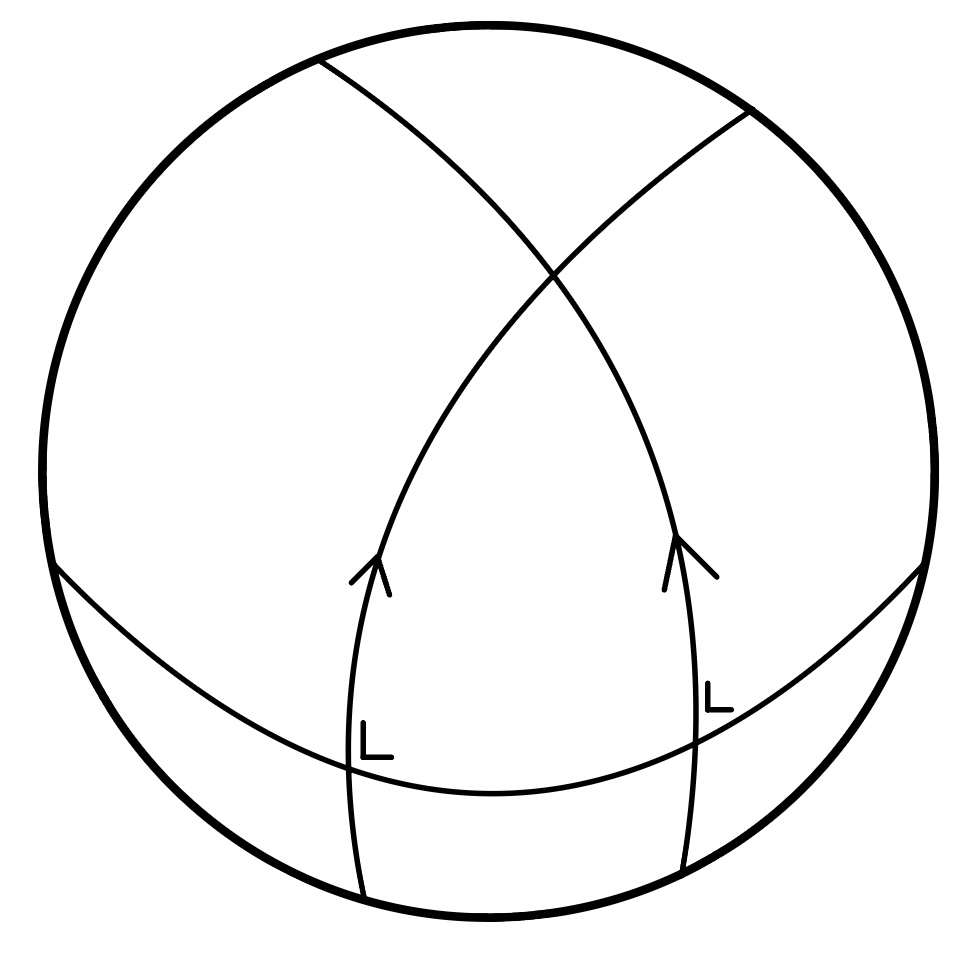
\includegraphics[scale=0.15]{Chapitres/5. Géodésiques/Images/sphere trajectoire qui se croise.jpg} 
\end{center}

\subsection{Le cas Newtonien}
On voudrait quantifier ce comportement dans un espace-temps courbe. Pour ce faire, on va d'abord étudier ce comportement dans un champ Newtonien. 

Une particule se déplaçant dans un champ de gravitation suit la trajectoire suivante :

\begin{equation}
    \frac{\td^2x^{i}}{\td t^2} = -\partial^{i}\Phi(x)
\end{equation}

Considérons à présent 2 particules voisines l'une en $x^{i}(t)$ et l'autre en $x^{i}(t) + \delta x^{i}(t)$. 

\begin{center} 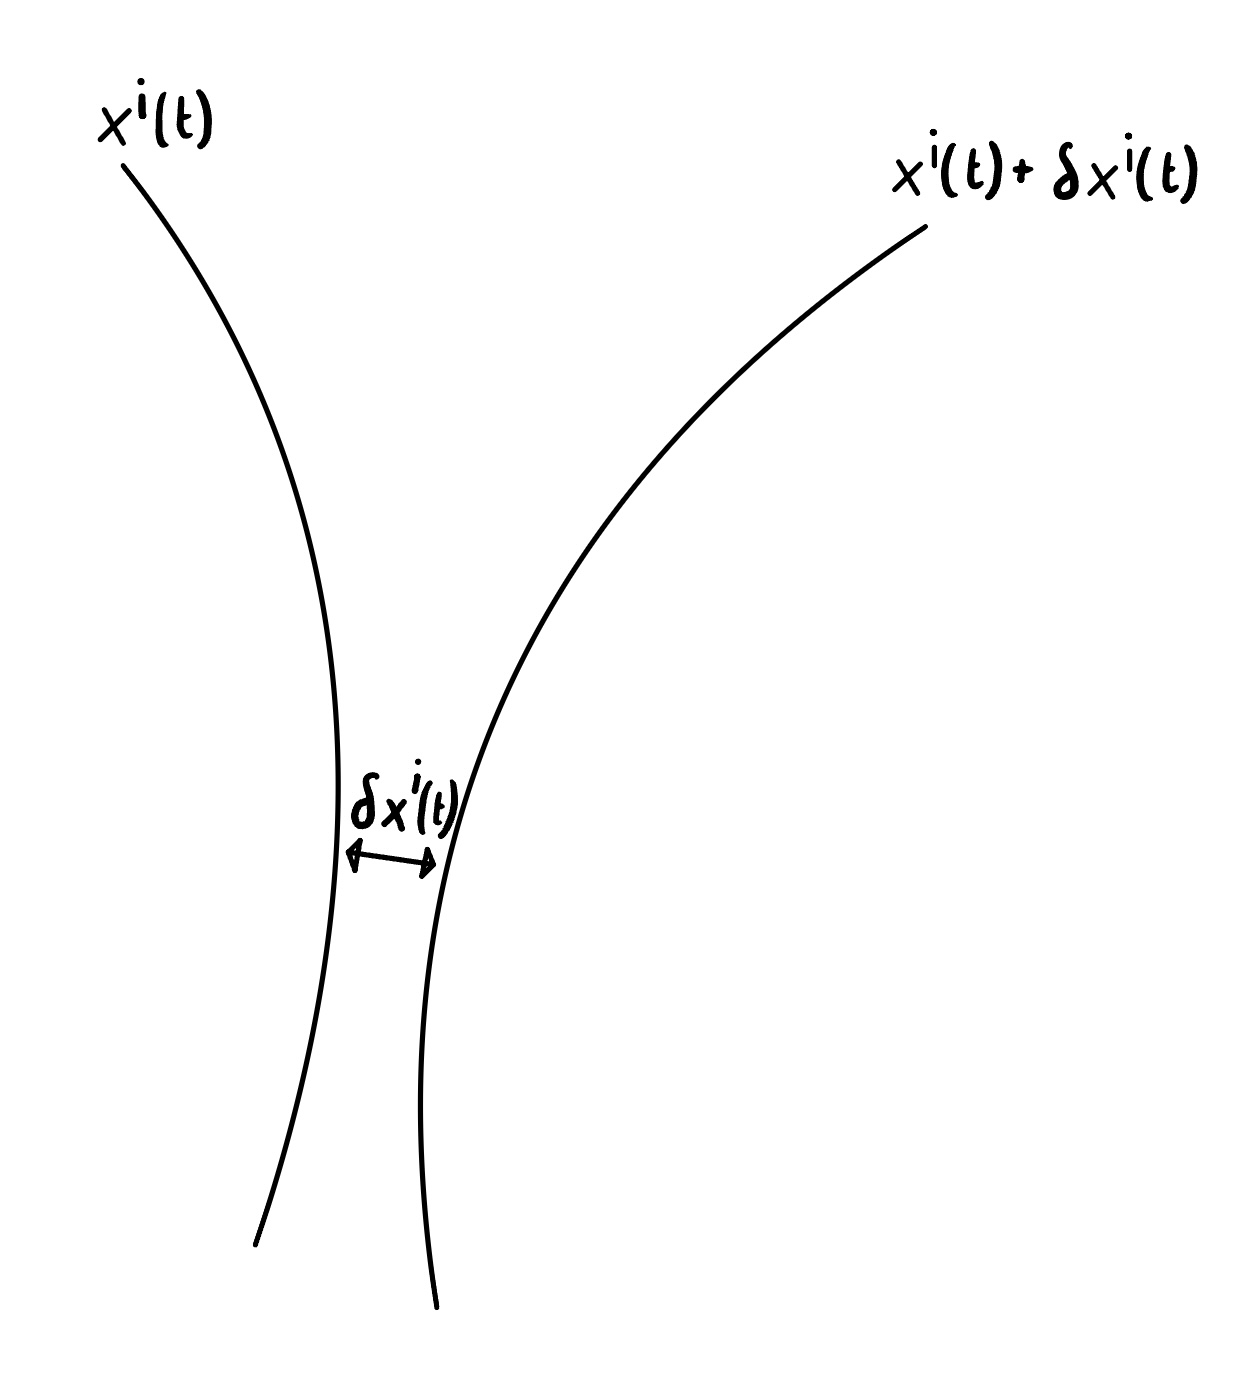
\includegraphics[scale=0.15]{Chapitres/5. Géodésiques/Images/mouvement infinitésimal.jpg} 
\end{center}

La deuxième particule obéit à l'équation suivante:

\begin{equation}
    \frac{\td ^2}{\td t^2}(x^{i}(t) + \delta x^{i}(t)) = -\partial^{i}\Phi(x + \delta x)
\end{equation}
On sait que 

\begin{equation}
    \frac{\td ^2}{\td t^2}(x^{i}(t) + \delta x^{i}(t))= \frac{\td ^2}{\td t^2}(x^{i}(t) ) + \frac{\td ^2}{\td t^2}(\delta x^{i}(t))
\end{equation}
Et on a aussi que

\begin{equation}
    \pd^i \Phi(x+\delta x) = \partial^{i}\Phi(x) + \partial_{j}(\partial^{i}\Phi(x))\delta x^{j}+\mathcal{O}(\delta x^2)
\end{equation}

On obtient donc
\begin{equation}
    \frac{\td ^2}{\td t^2}(\delta x^{i}(t)) = - \partial_{j}(\partial^{i}\Phi(x))\delta x^{j}
    \label{eq:forces de marées gravitationnelles}
\end{equation}
Cette équation décrit l'effet des forces de marées gravitationnelles (le gradient de la force gravitationnelle) sur une famille de 
particules se déplaçant dans un champ de gravitation.

\begin{center} 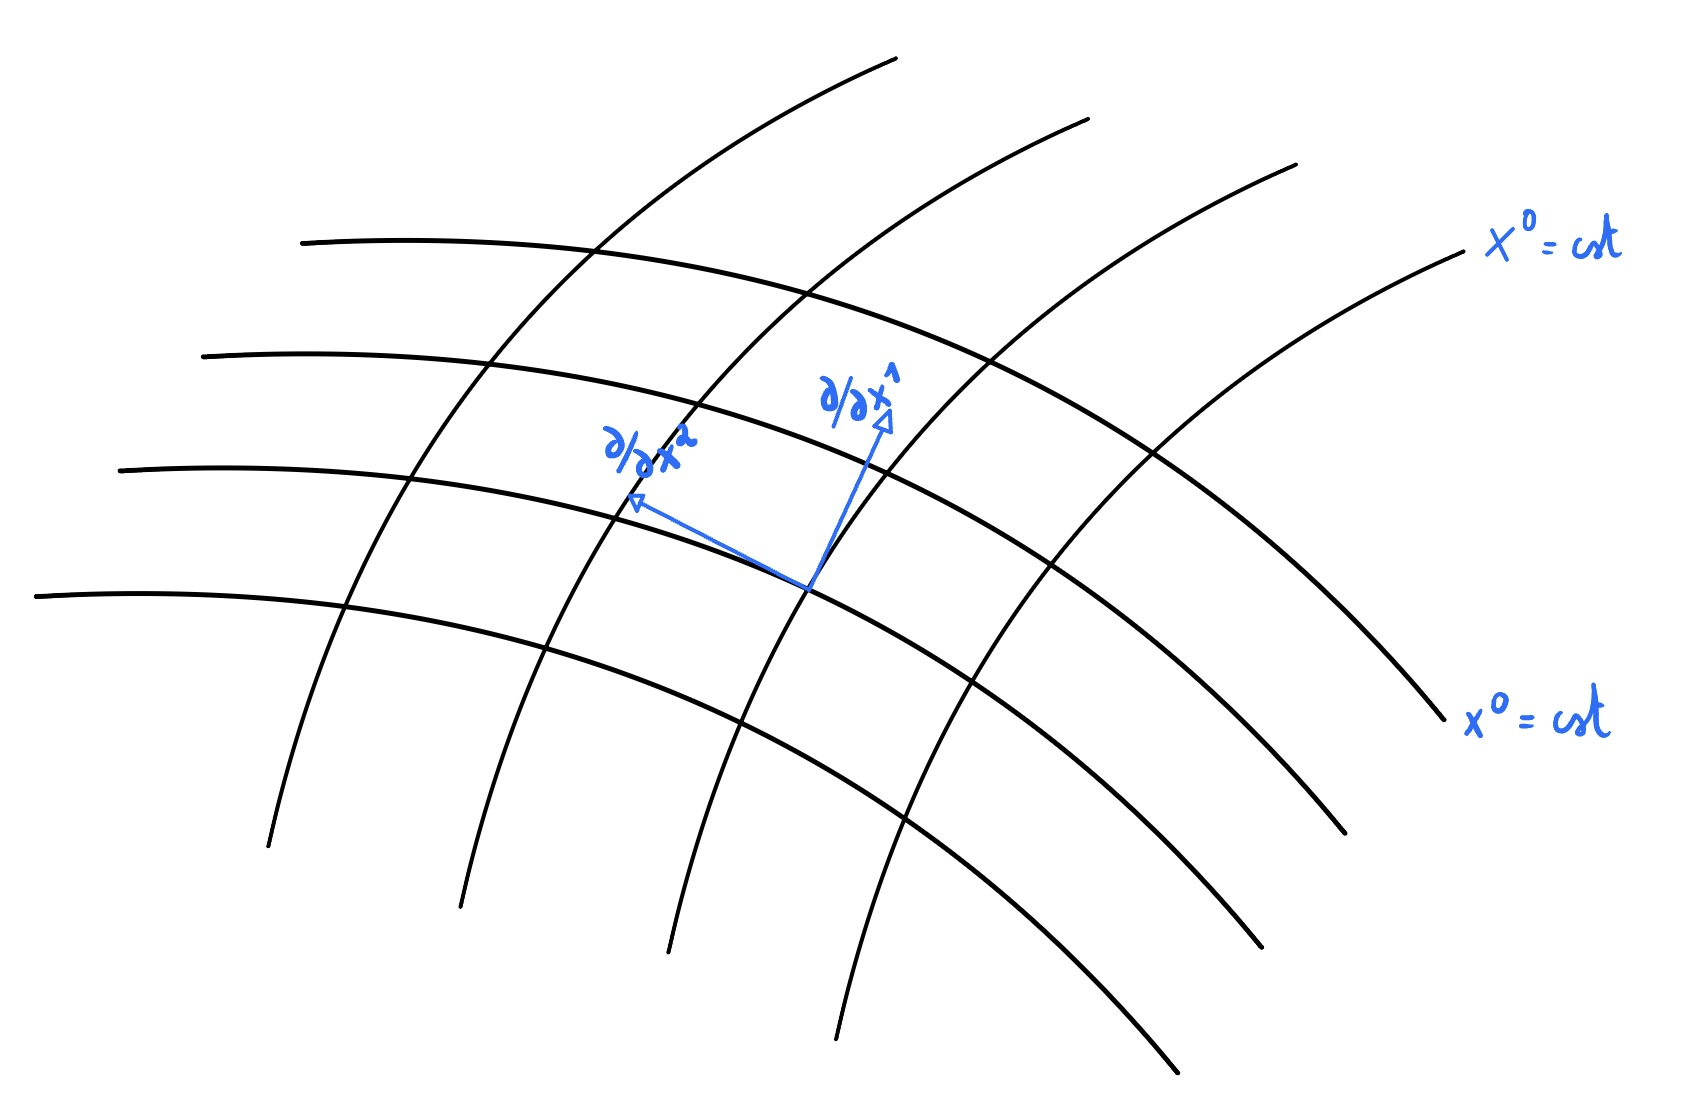
\includegraphics[scale=0.15]{Chapitres/5. Géodésiques/Images/courbure d'espace .jpg} 
\end{center}

\subsection{Généralisation covariante}
Considérons à présent un variété arbitraire $(\mathcal{M},g)$ munie de sa connexion de Levi-Civita. Soit une famille de géodésiques $\{\gamma_{s}(t)\}_s$ de paramètre affine $t$. Pour chaque valeur de $s$, on a une géodésique. Soit une carte locale et notons les champs tangents $T = T^{\mu}\partial_{\mu}$ d'une géodésique : 

\begin{equation}
    T^{\mu} = \left. \frac{\td x^{\mu}}{\td t}(\gamma_{s}(t))\right|_{s \text{ fixé}} = \frac{\pd x^{\mu}}{\pd t}(\gamma_{s}(t))
\end{equation}
qui est un champ tangent à la géodésique $s$. Par définition d'une géodésique, il est transporté parallèlement à lui-même:
\begin{equation}
    \nabla_{T}T = 0
\end{equation}
On définit également le \emph{déplacement} $S$ d'une géodésique à une géodésique voisine :
\begin{equation}
    S^{\mu} =\left. \frac{\td x^{\mu}}{\td s}(\gamma_{s}(t))\right|_{t \text{ fixé}}= \frac{\partial x^{\mu}}{\partial s}(\gamma_{s}(t))
\end{equation}
C'est la généralisation covariante de la séparation $\delta x^{i}$ utilisée auparavant. On voudrait calculer comment ce champ de vecteurs évolue lorsqu'on se déplace le long des géodésiques. On définit la vitesse relative des géodésiques par 

\begin{equation}
    V^{\mu} = (\nabla_{T}S)^{\mu} = T^{\rho}\nabla_{\rho}S^{\mu} \equiv \frac{\mathrm{D}}{\td t}S^{\mu}
\end{equation}
où $\frac{\td }{\td t} = T^{\mu}\partial_{\mu} \rightarrow \frac{\mathrm{D} }{\td t} = T^{\mu}\nabla_{\mu}$. L'accélération relative est définie comme :

\begin{equation}
    A^{\mu} = (\nabla_{T}V)^{\mu}\equiv\frac{\mathrm{D} ^2}{\td t^2}S^{\mu}
\end{equation}
Nous souhaiterions calculer $A^\mu$ et nous montrerons que celle-ci est intrinsèque à la courbure et donc à la variété.
Le résultat sera la généralisation covariante de l'équation [\ref{eq:forces de marées gravitationnelles}]. Notons d"jà que lorsque $A^{\mu}=0$, la métrique est plate. 

\subsubsection{Calcul de $A^\mu$}
Notons d'abord que la famille de géodésiques $\gamma_{s}(t)$ balaye une surface bidimensionnelle (à paramètres $(s,t)$) sur la variété $\mathcal{M}$ qui forme une sous variété de dimensions $2$ de $\mathcal{M}$. L'espace tangent de cette sous variété a pour base les vecteurs $S$ et $T$ (en tout point $S$ et $T$ sont linéairement indépendant). C'est-à-dire que les champs de vecteurs $S^{\mu}$ et $T^{\mu}$ définissent localement une base de l'espace tangent à cette sous-variété. Autrement dit, chaque point de cette sous-variété est uniquement décrite par la donnée d'une paire $(s,t)$.
\begin{theoremframe}
    \begin{propri} 
        Le crochet de Lie
        \begin{equation}
            [S,T] = 0
        \end{equation}
        est nul.
    \end{propri}
\end{theoremframe}
\begin{proof}

Rappelons que le crochet de Lie est défini comme
\begin{equation}
[S,T] \equiv S^{\mu}\partial_{\mu}T^{\nu} - T^{\alpha}\partial_{\alpha}S^{\nu}
\end{equation}
Considérons donc que les champs de vecteurs:

$$S = \frac{\partial}{\partial_{s}}$$, $$T = \frac{\partial}{\partial_{t}}$$

sont dans un système de coordonnées où $[S, T] = 0$. Comme le crochet de Lie est un champ de vecteurs (se transforme de manière covariante), si le commutateur est nul dans un système de coordonnée, il est nul dans tout système de coordonnée.
\end{proof}
\begin{theoremframe}
    \begin{propri}
        Pour une connexion sans torsion, on a que 

        \begin{equation}
            [S,T] = S^{\mu}\partial_{\mu}T^{\nu} - T^{\alpha}\partial_{\alpha}S^{\nu} = S^{\mu}\nabla_{\mu}T^{\nu} - T^{\alpha}\nabla_{\alpha}S^{\nu}
        \end{equation}
    \end{propri}
\end{theoremframe}
\begin{proof}
On peut prouver cette égalité de deux manières différentes. Soit on remarque que cette objet est tensoriel et alors on peut évaluer cette égalité dans un système de coordonnées localement inertiel. Dans un telle système de coordonnées on avait vu que $\nabla = \partial$. 

Sinon, on peut également calculer explicitement $S^{\mu}\nabla_{\mu}T^{\nu} - T^{\alpha}\nabla_{\alpha}S^{\nu}$. En développent, les termes en $\Gamma$ vont s'annuler pour une connexion sans torsion et il restera uniquement les termes avec les dérivées partielles, ce qui prouve l'identité.
\end{proof}
Ces deux propriétés impliquent

\begin{equation}
    S^{\mu}\nabla_{\mu}T^{\nu} - T^{\alpha}\nabla_{\alpha}S^{\nu} = 0
    \label{eq:champ de vecteur S et T}
\end{equation}
L'accelération s'écrit alors
\begin{align}
    A^{\mu} &= T^{\rho}\nabla_{\rho}(T^{\sigma}\nabla_{\sigma}S^{\mu})\\
    \intertext{Par l'équation \ref{eq:champ de vecteur S et T} :}
    &= T^{\rho}\nabla_{\rho}(S^{\sigma}\nabla_{\sigma}T^{\mu})\\
    \intertext{Par la règle de Leibniz}
    &= \textcolor{purple}{T^{\rho}\nabla_{\rho}S^{\sigma}} \nabla_{\sigma}T^{\mu} + T^{\rho}S^{\sigma}(\textcolor{blue}{\nabla_{\rho}\nabla_{\sigma}}T^{\mu})\\
    &= \textcolor{purple}{S^\rho \nabla_\rho T^\sigma} \nabla_\sigma T^\mu +T^{\rho}S^{\sigma}(\textcolor{blue}{[\nabla_{\rho},\nabla_{\sigma}]}T^{\mu}) +T^{\rho}S^{\sigma}(\textcolor{blue}{\nabla_{\sigma}\nabla_{\rho}}T^{\mu}) 
    \intertext{Or, comme $[\nabla_{\rho}, \nabla_{\sigma}]T^{\mu} = R^{\mu}_{\alpha \rho \sigma}T^{\alpha}$ :}
    &= S^{\rho}\nabla_{\rho}T^{\sigma}\nabla_{\sigma}T^{\mu}+ T^{\rho}S^{\sigma}\nabla_{\sigma}\nabla_{\rho}T^{\mu} + T^{\rho}S^{\sigma}R\indices{^{\mu}_{\alpha \rho \sigma}} T^{\alpha}
\end{align}
Une intégration par parties donne alors 
\begin{align}
    T^{\rho}S^{\sigma}\nabla_{\sigma}\nabla_{\rho}T^{\mu} = S^{\sigma}\nabla_{\sigma}(T^{\rho}\nabla_{\rho}T^{\mu}) - S^{\sigma}\nabla_{\sigma}T^{\rho}\nabla_{\rho}T^{\mu}
\end{align}
Or, $S^{\sigma}\nabla_{\sigma}(T^{\rho}\nabla_{\rho}T^{\mu}) = \nabla_S \nabla_T T^\mu 0$ (pour une géodésique $\nabla_{T} T=0$). On réécrit alors
\begin{align}
     A^{\mu} &=S^{\rho}\nabla_{\rho}T^{\sigma}\nabla_{\sigma}T^{\mu}- S^{\sigma}\nabla_{\sigma}T^{\rho}\nabla_{\rho}T^{\mu}+ T^{\rho}S^{\sigma}R\indices{^{\mu}_{\alpha \rho \sigma}}T^{\alpha}\\
     &=T^{\rho}S^{\sigma}R\indices{^{\mu}_{\alpha \rho \sigma}} T^{\alpha}
\end{align}
Finalement, on obtient que 

\begin{equation}
    \boxed{A^{\mu} = T^{\rho}S^{\sigma}R\indices{^{\mu}_{\alpha \rho \sigma}}T^{\alpha}}
\end{equation}
Cette équation est appelé équation de déviation géodésique (ou équation de Jacobi). 
On remarque que l'accélération relative est complètement capturée par le tenseur de Riemann, qui est une quantité intrinsèque à la variété\footnote{Peut être définie sans nécessiter un espace ambiant dans lequel est plongée la variété (comme p.ex. une surface $S \subset \R^3$). En effet, la métrique elle-même peut être définie de manière intrinsèque, et le tenseur de Riemann pour une connexion de Levi-Civita est uniquement déterminée à partir de la métrique.} et qui caractérise la courbure de celle-ci. Le tenseur de Riemann est donc responsable de l'accélération relative de 2 géodésiques voisines. 
\begin{exmp}
    Dans un espace plat, $R^{\mu}_{\alpha \rho \sigma} = 0$ et donc $A^{\mu} =0$. Ainsi :
    \begin{equation}
        S^{\mu} = \delta x^{\mu}(t) = C^{\mu}t + D^{\mu}
    \end{equation}
où $C$ et $D$ sont des constantes. Ainsi $S^{\mu}$ est une fonction linéaire du temps. On retrouve les axiomes d'Euclide qui dit que 2 lignes droites s'intersectent au plus une fois et que 2 droites parallèles ne peuvent pas s'intersecter.
\end{exmp}
